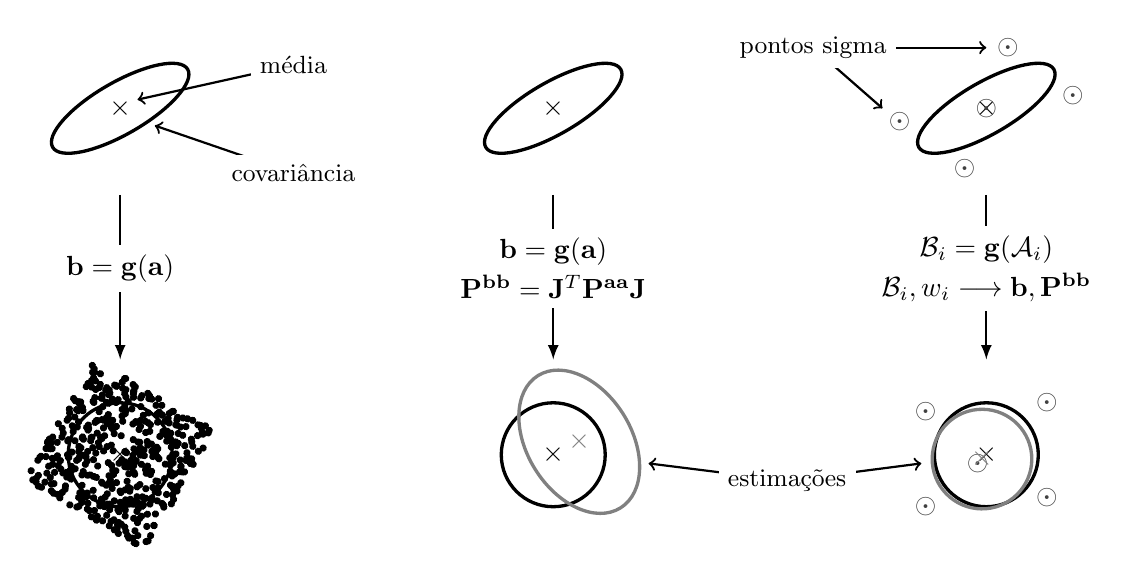
\begin{tikzpicture}[scale=1.1]
    \begin{scope}[rotate=-60]
        \draw plot[mark=*, only marks, mark size=1] file {data/unscented-cloudx.dat};
    \end{scope}

    \pgfmathsetseed{64698676}
    \draw plot[mark=*, only marks, mark size=1, samples=500, rotate around={60:(0, -4)}] ({0.8*rand}, {-4 + 0.8*rand});

    \foreach \i in {0,5,10} {
        \node[black] at (\i, 0) {$\bm{\times}$};
        \draw[very thick, black, rotate around={-60:(\i, 0)}] (\i, 0) ellipse (0.3 and 0.9);
        \node[black] at (\i, -4) {$\bm{\times}$};
        \draw[very thick, black] (\i, -4) circle (0.6);
    }

    \draw[-latex, thick] (0, -1) -- (0, -2.9);
    \node[fill=white] at (0, -1.85) {$\mathbf{b} = \mathbf{g}(\mathbf{a})$};

    % Linearized
    \draw[very thick, gray, rotate around={32:((5.3, -3.85))}] (5.3, -3.85) ellipse (0.6 and 0.9);
    \node[gray] at (5.3, -3.85) {$\bm{\times}$};

    \draw[-latex, thick] (5, -1) -- (5, -2.9);
    \node[fill=white, align=center] at (5, -1.85) {$\Bar{\mathbf{b}} = \mathbf{g}(\Bar{\mathbf{a}})$\\[2.5pt]$\mathbf{P}^{\mathbf{b}\mathbf{b}} = \mathbf{J}^T \mathbf{P}^{\mathbf{a}\mathbf{a}} \mathbf{J}$};

    % UT
    \draw[very thick, gray, rotate around={5:((9.95, -4.05))}] (9.95, -4.05) circle (0.575);
    \node[darkgray] at (10, 0) {$\bm{\odot}$};
    \node[darkgray] at (9.9, -4.1) {$\bm{\odot}$};
    \foreach \i in {-1, 1} {
        \node[darkgray] at (10 + 1*\i, 0.15*\i) {$\bm{\odot}$};
        \node[darkgray] at (10 + 0.25*\i, 0.7*\i) {$\bm{\odot}$};
        \node[darkgray] at (10 - 0.7*\i, -4 + 0.5*\i) {$\bm{\odot}$};
        \node[darkgray] at (10 + 0.7*\i, -4 + 0.6*\i) {$\bm{\odot}$};
    }
    \node[gray] at (9.95, -4.05) {$\bm{\times}$};

    \draw[-latex, thick] (10, -1) -- (10, -2.9);
    \node[fill=white, align=center] at (10, -1.85) {$\bm{\mathcal{B}}_i = \mathbf{g}(\bm{\mathcal{A}}_i)$\\[2.5pt]$\bm{\mathcal{B}}_i, w_i \longrightarrow \Bar{\mathbf{b}}, \mathbf{P}^{\mathbf{b}\mathbf{b}}$};

    \draw[->, thick] (2, 0.5) -- (0.2, 0.1);
    \draw[->, thick] (2, -0.75) -- (0.4, -0.2);
    \node[fill=white, align=center] at (2, 0.5) {\small média};
    \node[fill=white, align=center] at (2, -0.75) {\small covariância};

    \draw[->, thick] (7.7, -4.3) -- (6.1, -4.1);
    \draw[->, thick] (7.7, -4.3) -- (9.25, -4.1);
    \node[fill=white, align=center] at (7.7, -4.3) {\small estimações};

    \draw[->, thick] (8, 0.7) -- (10, 0.7);
    \draw[->, thick] (8, 0.7) -- (8.8, 0);
    \node[fill=white, align=center] at (8, 0.7) {\small pontos sigma};
\end{tikzpicture}
